\section{Introduction}

Personal AI systems increasingly promise long-term memory, user adaptation, personalized dialogue, and digital-twin-like behavior \cite{park2023generative,li2016persona,zhang2018personalizing,zhong2023memorybank,packer2023memgpt,zhang2024memorysurvey}. For such systems, it is not enough to produce a plausible description of a user or to imitate surface style. A useful personal agent should preserve behavioral continuity: when placed back into a historical context, it should predict what the user is likely to do next.

This paper studies that problem in the concrete setting of personal GPT chat logs. A long history of user--assistant interactions contains stable preferences, changing goals, unresolved tasks, and topic shifts. However, evaluating whether a model has captured those factors is difficult. Free-form response generation metrics are brittle; persona summaries are hard to verify; and using the full history in-context makes it unclear whether improvement comes from structured user modeling or raw retrieval. Similar concerns appear in personalization, social-simulation, and population-simulation benchmarks \cite{salemi2023lamp,zhou2023sotopia,wang2024sotopiapi,argyle2023outofone}. We therefore focus on a narrower but measurable question: can a system predict the user's next conversational action in held-out historical replay?

We propose a proxy replay benchmark for this setting. Each example consists of a conversation context, a target user turn, and a rule-derived action label such as \emph{request how-to}, \emph{compare options}, \emph{provide more context}, or \emph{topic shift}. The representation is explicit: persona facts, dynamic state, and memory nodes are materialized as intermediate objects rather than hidden inside a prompt. This setup lets us test which part of the representation is actually useful under held-out replay, and whether a lexical retrieval baseline is already stronger than a learned state router.

We organize the study around three questions. \textbf{RQ1}: does state-aware information improve held-out replay over a no-state baseline? \textbf{RQ2}: does a learned state selector improve over a heuristic state mapper? \textbf{RQ3}: does state routing add signal beyond strong lexical similarity? These questions evaluate a narrow proxy for behavioral continuity rather than broad human simulation.

Our main finding is nuanced. After tightening the proxy \texttt{topic\_shift} label, a lexical context NN baseline using CJK-aware character n-gram similarity achieves the highest accuracy and macro-F1 (0.35 / 0.38), while the learned state router scores 0.23 / 0.30. We do not detect a significant paired accuracy difference (McNemar $p=0.074$), but bootstrap CIs are wide at $n=40$. Critically, adding state routing to the lexical baseline changes zero predictions (40/40 identical). State-only gains in earlier prototypes were artifacts of a weak similarity metric.

This paper makes four contributions:
\begin{enumerate}
    \item We define a proxy next-action replay task for personal GPT chat logs, making behavioral continuity measurable.
    \item We implement an explicit persona/state/memory pipeline and use leakage-free ablations to test the dynamic-state component.
    \item We show that a CJK-aware lexical retrieval baseline performs best, exceeding both a learned state router and pretrained embedding models; state routing adds zero signal on top of lexical or embedding similarity.
    \item We identify two pitfalls: state-prior baselines can inflate accuracy while collapsing macro-F1, and state-routing gains must be validated against strong lexical comparators with uncertainty estimates.
\end{enumerate}

Figure~\ref{fig:overview} summarizes the replay setup and evaluation path.

\begin{figure}[t]
\centering
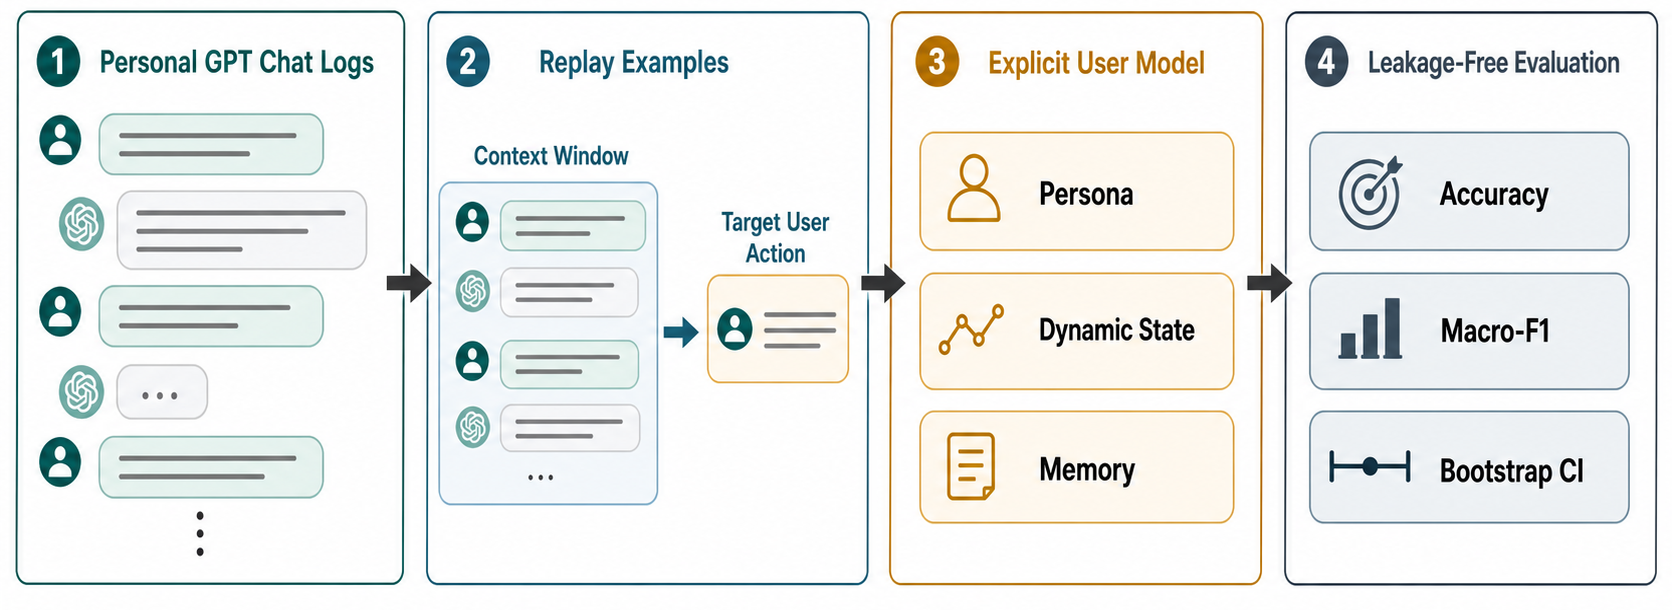
\includegraphics[width=0.96\linewidth]{figures/paper_overview_cropped.png}
\caption{Paper overview: chat logs are normalized into replay examples, mapped into explicit user representations, and evaluated with leakage-free held-out metrics.}
\label{fig:overview}
\end{figure}

The claim is deliberately scoped: the benchmark uses one user's GPT logs with rule-derived proxy labels and a small held-out set ($n=40$), so the results do not establish a complete digital twin or general human simulator. They show that state-aware replay is auditable, and that bootstrap CIs and paired tests are necessary for small replay benchmarks.
